\section{Configuración funcional - Organización de la empresa}
\subsection{Autoevaluación}
En esta sección se han cumplido los objetivos correspondientes al 10.
\subsection{Introducción}
Este módulo se enfoca en la gestión y la organización de la empresa que Odoo nos permite realizar. Se va a describir como se ha creado una nueva compañía, la distribución de usuarios entre las entidades y la organización estructural de la empresa. Además, de explora la internacionalización en Odoo, donde se prueba el soporte multilingüe y el manejo de distintas monedas .
\subsection{Metodología}
\paragraph{}
En cuanto a la creación de una nueva compañía, el proceso ha comenzado accediendo al menú de configuración dentro de las opciones generales. Luego, se ha hecho clic en el enlace \textit{Administrar compañías} para iniciar el proceso de creación de la empresa. Posteriormente, se ha completado el formulario correspondiente. Después, se ha navegado hasta el menú de \textit{Ramas de la compañía} para gestionar las sucursales de la compañía matriz recién creada, agregando dos nuevas: CochesMA.UK y CochesMA.US
\paragraph{}
Además, se ha procedido a gestionar los usuarios para las compañías creadas, tanto la matriz como las sucursales. Para ello, en las opciones generales de los ajustes de Odoo, se ha pulsado en \textit{Administrar usuarios}. Desde este menú se han creado 9 usuarios, seleccionando \textit{Nuevo} y completando el formulario correspondiente. Es importante destacar que se puede seleccionar a qué compañías tiene acceso cada usuario. Además, se puede cambiar el idioma para el usuario desde el menú de preferencias. En caso de que el idioma deseado no aparezca, se ha pulsado en el icono del mundo para buscarlo.
\paragraph{}
Por otro lado, Odoo ofrece herramientas de internacionalización, incluyendo soporte multilingüe. Para configurarlo, se ha accedido a las opciones generales de los ajustes, donde se ha seleccionado \textit{Añadir idiomas} y se han escogido los idiomas deseados. También es posible establecer varias monedas dentro de la compañía. Para ello, se ha seleccionado la compañía matriz en la opción de \textit{Administración de compañías} dentro de las opciones generales, y en la sección de \textit{Moneda} se han activado las monedas que se desean utilizar tanto en la matriz como en las sucursales. Finalmente, se ha seleccionado la moneda que se utilizará como predeterminada.
\subsection{Resultados y análisis}
Se ha llevado a cabo el proceso de creación de una compañía matriz llamada CochesMA la cual tiene dos compañías rama, una en Reino Unido llamada CochesMA.UK y otra en Estados Unidos llamada CochesMA.US.
\begin{figure}[h]
    \centering
    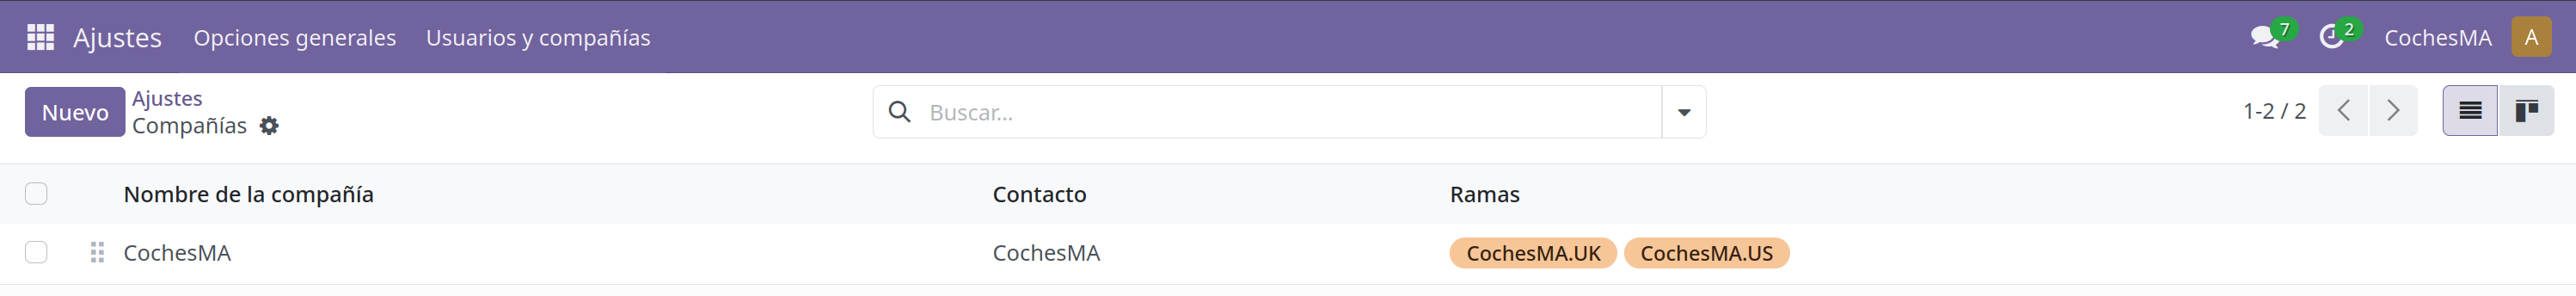
\includegraphics[width=\linewidth]{fotosConfiguración/estructuraEmpresarial.png}
    \caption{Compañía matriz con sus dos compañías rama}
    \label{fig:enter-label}
\end{figure}
\begin{figure}[h]
    \centering
    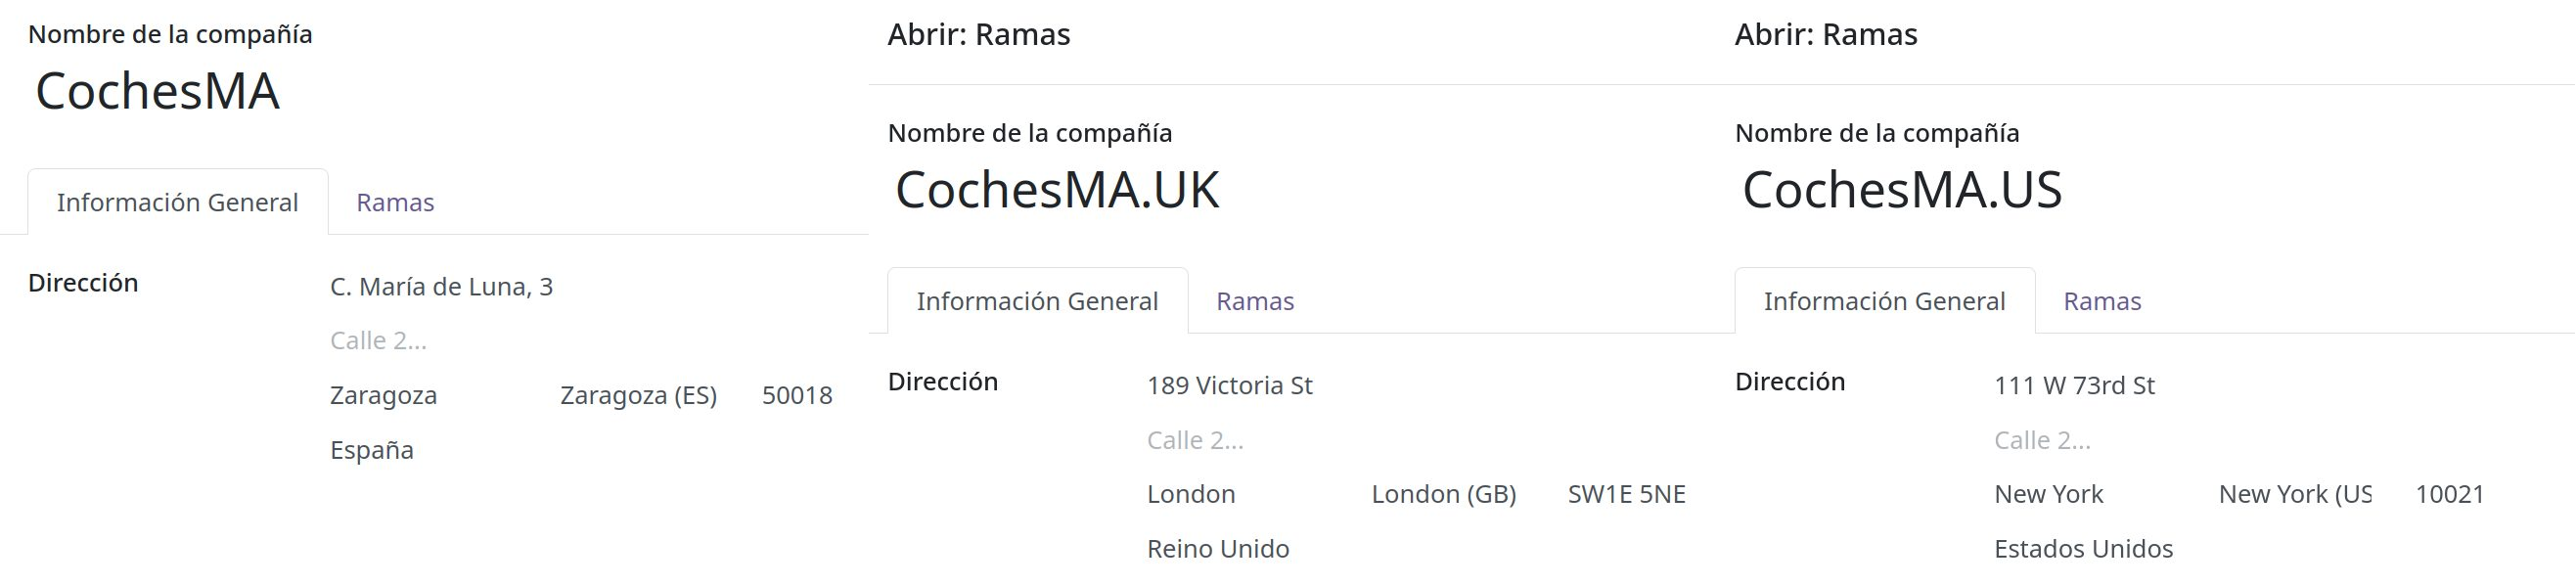
\includegraphics[width=\linewidth]{fotosConfiguración/ubicaciones.jpg}
    \caption{Ubicaciones de las compañias}
    \label{fig:enter-label}
\end{figure}
Se han creado 9 usuarios. John, James, Marcus, Mark, Sheila y Tom hablan ingles y Juan, Maria y Pedro hablan español. John, James y Pedro pertenecen a la compañía matriz. Juan, Marcus y Sheila pertenecen a la rama de Estados Unidos. Maria, Mark y Tom pertenecen a la rama de Reino Unido.
Además, se han añadido los idiomas de los usuarios a Odoo y se ha establecido la siguiente la moneda principal el Euro, pero se ha permitido el uso de la Libra esterlina para CochesMA.UK y el Dolar estadounidense para CochesMA.US. 
\begin{figure}[h]
    \centering
    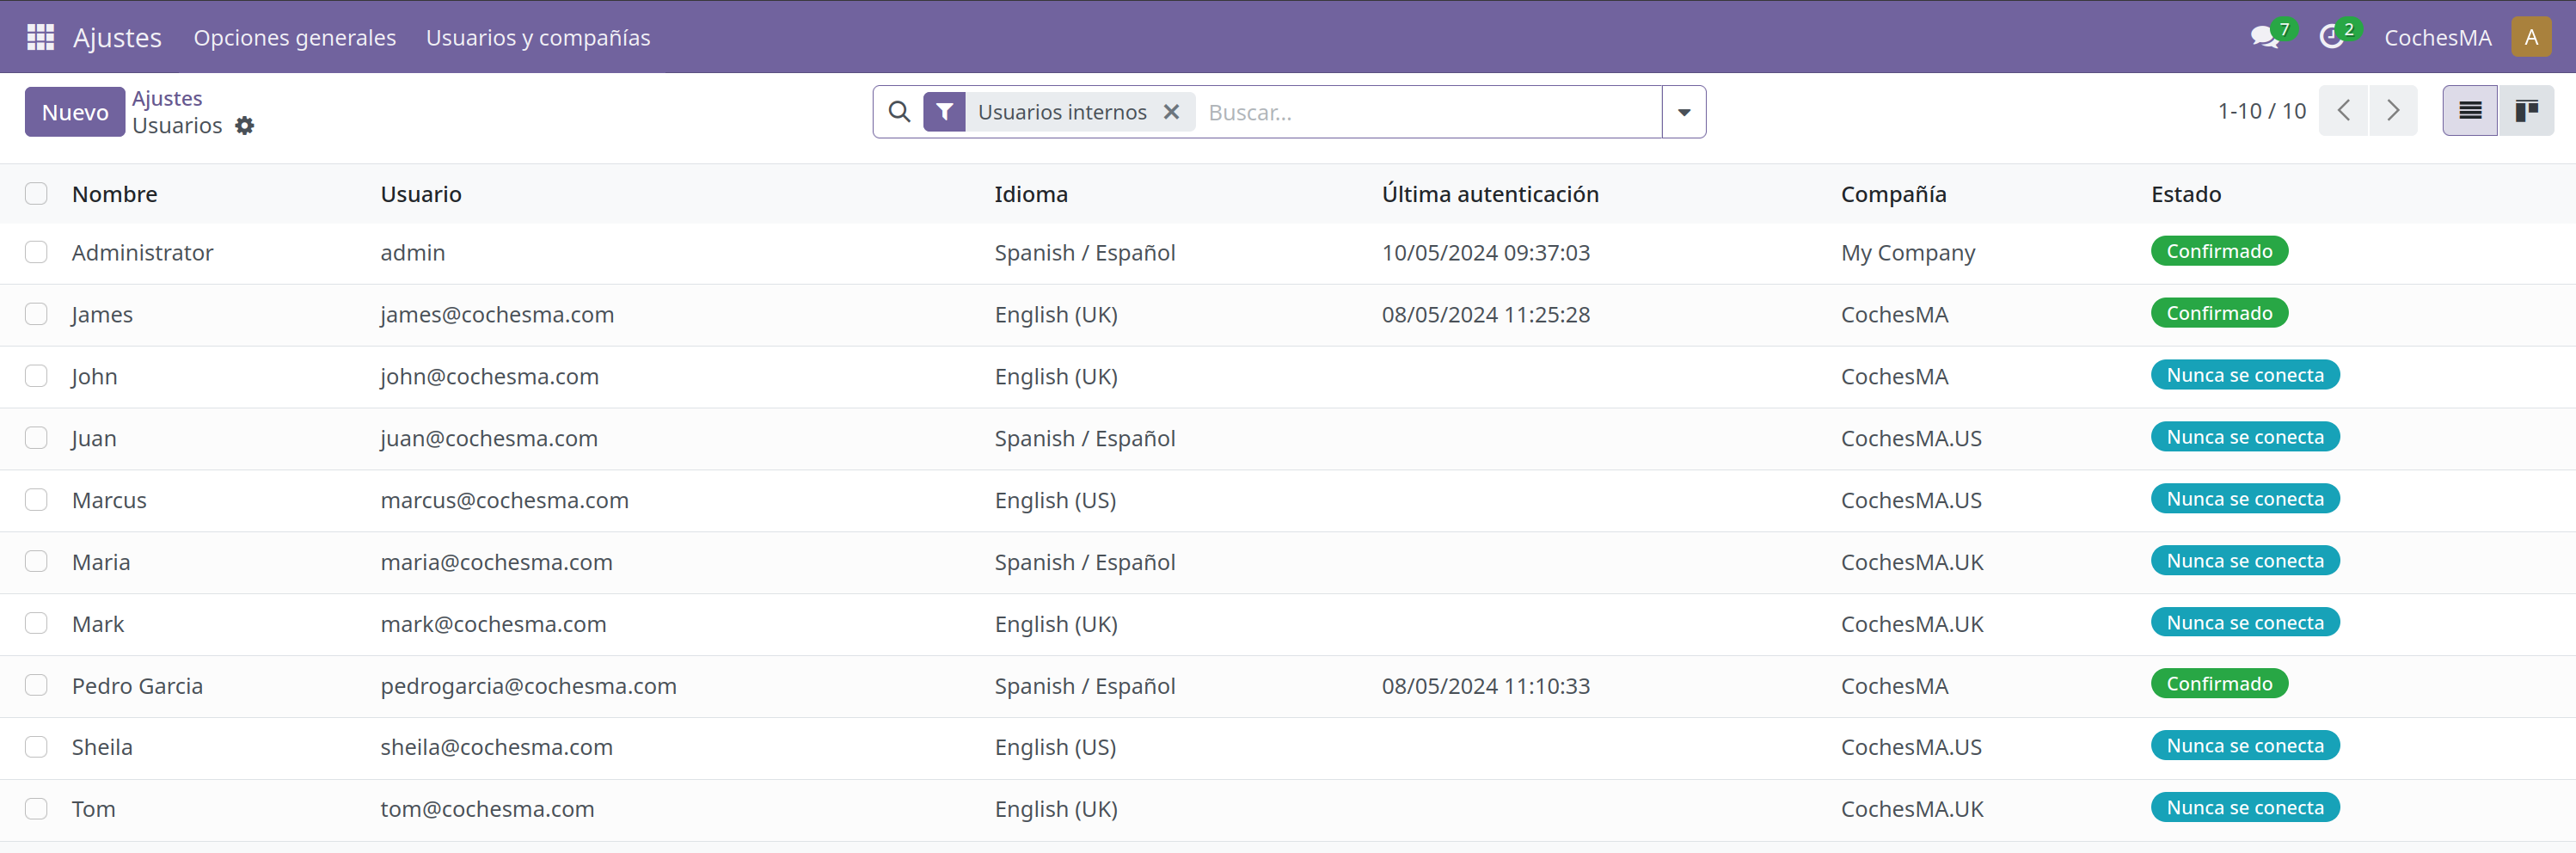
\includegraphics[width=\linewidth]{fotosConfiguración/usuarios.png}
    \caption{Usuarios creados con su idioma y compañía}
    \label{fig:enter-label}
\end{figure}

\begin{figure}[h]
    \centering
    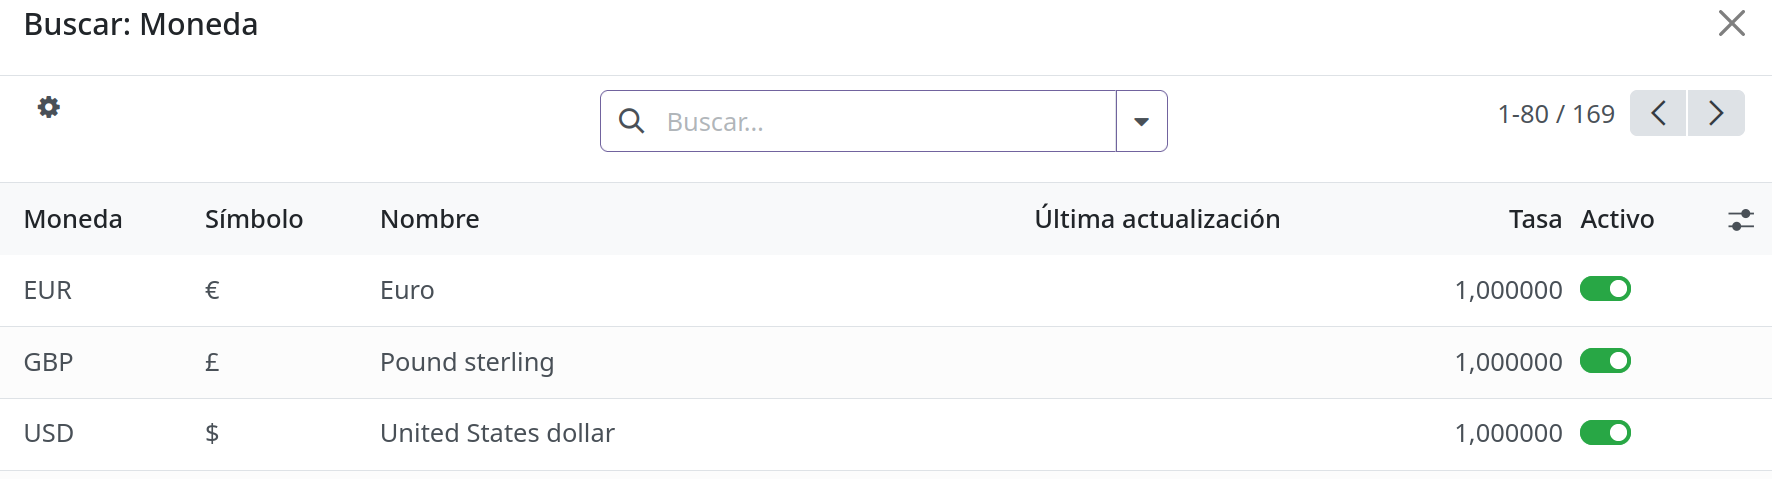
\includegraphics[width=\linewidth]{fotosConfiguración/divisas.png}
    \caption{Divisas de las compañías}
    \label{fig:enter-label}
\end{figure}
\subsection{Conclusiones}
La capacidad de Odoo para gestionar múltiples compañías se demuestra en la capacidad que tiene para adaptarse a estructuras empresariales con empresas matrices y ramas.
En cuanto al proceso de creación de usuarios en Odoo es sencillo y permite especificar detalles como la compañía a la que pertenecen, su acceso a los módulos y su idioma preferido, agilizando así el proceso de integración. La posibilidad de añadir nuevos idiomas al sistema de forma sencilla mejora la experiencia del usuario y facilita la comunicación en entornos internacionales.
Sin embargo, es importante tener en cuenta que, aunque la creación de una nueva compañía y la gestión de sus ramas se realiza de manera intuitiva, la gestión de múltiples monedas puede resultar un poco más oculta. Para activar las monedas, es necesario pulsar en \textit{Buscar más}, y existen ciertas restricciones, como la obligación de que las empresas filiales tengan la misma moneda que la matriz.
En general, son aspectos básicos del sistema que son fáciles de configurar aunque tienen gran importancia ya que son la base sobre la que se construirán las personalizaciones de los siguientes módulos.
\newpage
\section{Configuración funcional - Imagen corporativa}
\subsection{Autoevaluación}
En esta sección se han cumplido los objetivos correspondientes al 10.
\subsection{Introducción}
Este apartado se enfoca en mejorar la presencia digital de la empresa. Inicia con la activación del sistema multilingüe en la web, para posibilitar un alcance global. También, se aborda la personalización de la página web, integrando la información de la empresa y el logo y ajustando el tema y los colores para alinearla con la imagen de la empresa. Además, se realizan optimizaciones SEO para mejorar la visibilidad de la web en los motores de búsqueda y la implementación de SSL para garantizar la seguridad.
\subsection{Metodología}
\paragraph{}
Para probar el sistema multilingüe de la web hay que asegurase que los idiomas deseados están en el apartado de sitio web de la configuración y si no añadirlo desde ahí, cabe destacar que sólo dejará añadir idiomas que tengan los usuarios de la compañía. Una vez realizado este paso, el usuario podrá cambiar el idioma en la web desde la esquina superior izquierda o en el pie de página. 
\paragraph{}
Además, se ha llevado a cabo la personalización de la página web para incluir la información de la empresa. Para ello, se ha accedido al modo de edición navegando a la página web y seleccionando el modo de edición. Se ha ido a la página \textit{Contáctenos}, se ha editado haciendo haciendo doble clic en el bloque de la geolocalización y se ha introducido la información de la dirección, el correo electrónico y el teléfono, al igual que en el pie de página que es común en muchas páginas de la web. Además, en la pantalla \textit{Home} de la página web se ha editado el bloque de la misión y el bloque de Acerca de en el pie de página de la misma manera. 
\paragraph{}
Por otro lado, también se puede cambiar tanto los colores como el tema de la web. Para ello, se debe estar en el modo edición en la web y seleccionar el menú \textit{Tema} en la barra lateral derecha. A continuación, se puede cambiar los colores tanto principales como secundarios del tema, sustituyendo los colores por otros. Si se quiere cambiar de tema, se ha hecho clic en \textit{Cambiar tema} y se ha seleccionado el nuevo tema entre los disponibles. También, se ha añadido el logo a la página web haciendo clic en el logo predeterminado. Se ha desplegado la barra lateral derecha, se ha hecho clic en \textit{Reemplazar} y se ha seleccionado el nuevo logo. En los ajustes del sitio web se ha añadido el logo en la opción de \textit{Favicon} para que también se muestre el logo en la parte superior de la pestaña en el buscador. 
\paragraph{}
Para mejorar el ranking de búsqueda con Google se han utilizado las herramientas SEO. En este menú se ha editado el título y la descripción y se ha añadido el logo para que aparezca desde el buscador. También, incluye la posibilidad de utilizar la herramienta de palabras clave, se han añadido un conjunto de palabras en la web para que cuando los usuarios busquen estas palabras aparezca nuestra web.

\paragraph{}
Una vez que hemos realizado la web hemos configurado la web de nuestra empresa en un dominio propio con acceso seguro SSL. Esta paso es esencial a la hora de determinar si este ERP es adecuado para nuestra empresa. Ya que es una funcionalidad que se va a necesitar de cara a permitir el acceso a nuestros clientes y usuarios desde cualquier navegador de forma segura. Esta configuración se ha realizado de forma local para realizar el análisis. La máquina utilizada para realizar las pruebas es un MacBook Pro de 2018 con un procesador Intel i5. El equipo a determinado que la mejor forma de montar un servidor SSL localmente es utilizando \textit{Nginx} y Docker. Se ha planteado utilizar una máquina Ubuntu y seguir los pasos descritos en: \href{https://www.digitalocean.com/community/tutorials/how-to-create-a-self-signed-ssl-certificate-for-nginx-in-ubuntu-20-04-1}{How To Create a Self-Signed SSL Certificate for Nginx in Ubuntu 20.04}. Sin embargo, esta alternativa no era la mejor opción para nuestro objetivo y situación, ya que al tener Odoo desplegado en un contenedor Docker. Y esto nos permite modificar nuestro \textit{docker-compose.yml} añadiendo el servicio de Nginx, el cual nos proporciona el certificado SSL. 

\paragraph{}
Los pasos que hemos llevado a cabo para implementar un servidor SSL local en Odoo utilizando Docker Compose y Nginx han sido:\\
Lo primero que hemos realizado es generar un certificado SSL utilizando OpenSSL, el cual nos genera un par de claves públicas y privada, y un certificado autofirmado válido por un año. Para ello hemos abierto nuestra terminal y ejecutado el siguiente comando:

 \begin{lstlisting}[frame=single, basicstyle=\small]
openssl req -x509 -nodes -days 365 -newkey rsa:2048
-keyout localhost.key -out localhost.crt
\end{lstlisting}
\paragraph{}
Al ejecutarlo deberemos rellenar nuestro país, región, ciudad, nombre de la organización, nombre del departamento, nombre del dominio y un correo electrónico. Este par de claves las hemos almacenado en un directorio llamado \textit{certificados}. A continuación hemos modificado el fichero \textit{docker-compose.yml} que creamos para la instalación, obteniendo este nuevo fichero: 
\begin{lstlisting}[frame=single, basicstyle=\small]
version: "3.1"
services:
  odoo:
    image: odoo:17.0
    depends_on:
      - db
    ports:
      - "8069:8069"
    volumes:
      - odoo-web-data:/var/lib/odoo
    environment:
      - HOST=db
      - USER=odoo
      - PASSWORD=myodoo

  db:
    image: postgres:13
    environment:
      - POSTGRES_DB=postgres
      - POSTGRES_PASSWORD=myodoo
      - POSTGRES_USER=odoo
      - PGDATA=/var/lib/postgresql/data/pgdata
    volumes:
      - odoo-db-data:/var/lib/postgresql/data/pgdata

  nginx:
    image: nginx:latest
    ports:
      - "443:443"
    volumes:
      - ./certificados:/certificados:ro
      - ./nginx.conf:/etc/nginx/nginx.conf:ro
    depends_on:
      - odoo

volumes:
  odoo-web-data:
  odoo-db-data:
\end{lstlisting}

\paragraph{}
Además de este fichero debemos crear un llamado \textit{nginx.conf} en el cual definiremos la configuración básica de Nginx para SSL. Una vez que tenemos ambos ficheros correctamente configurados podemos iniciar el contenedor desde la terminal, ejecutando en el directorio correcto el comando:
 \begin{lstlisting}[frame=single, basicstyle=\small]
docker-compose up -d
\end{lstlisting}
\paragraph{}
Por último, abrimos nuestro navegador y buscamos https://localhost. Si hemos realizado todos los pasos correctamente nos tendrá que aparecer el siguiente mensaje: 
\begin{figure}[h]
    \centering
    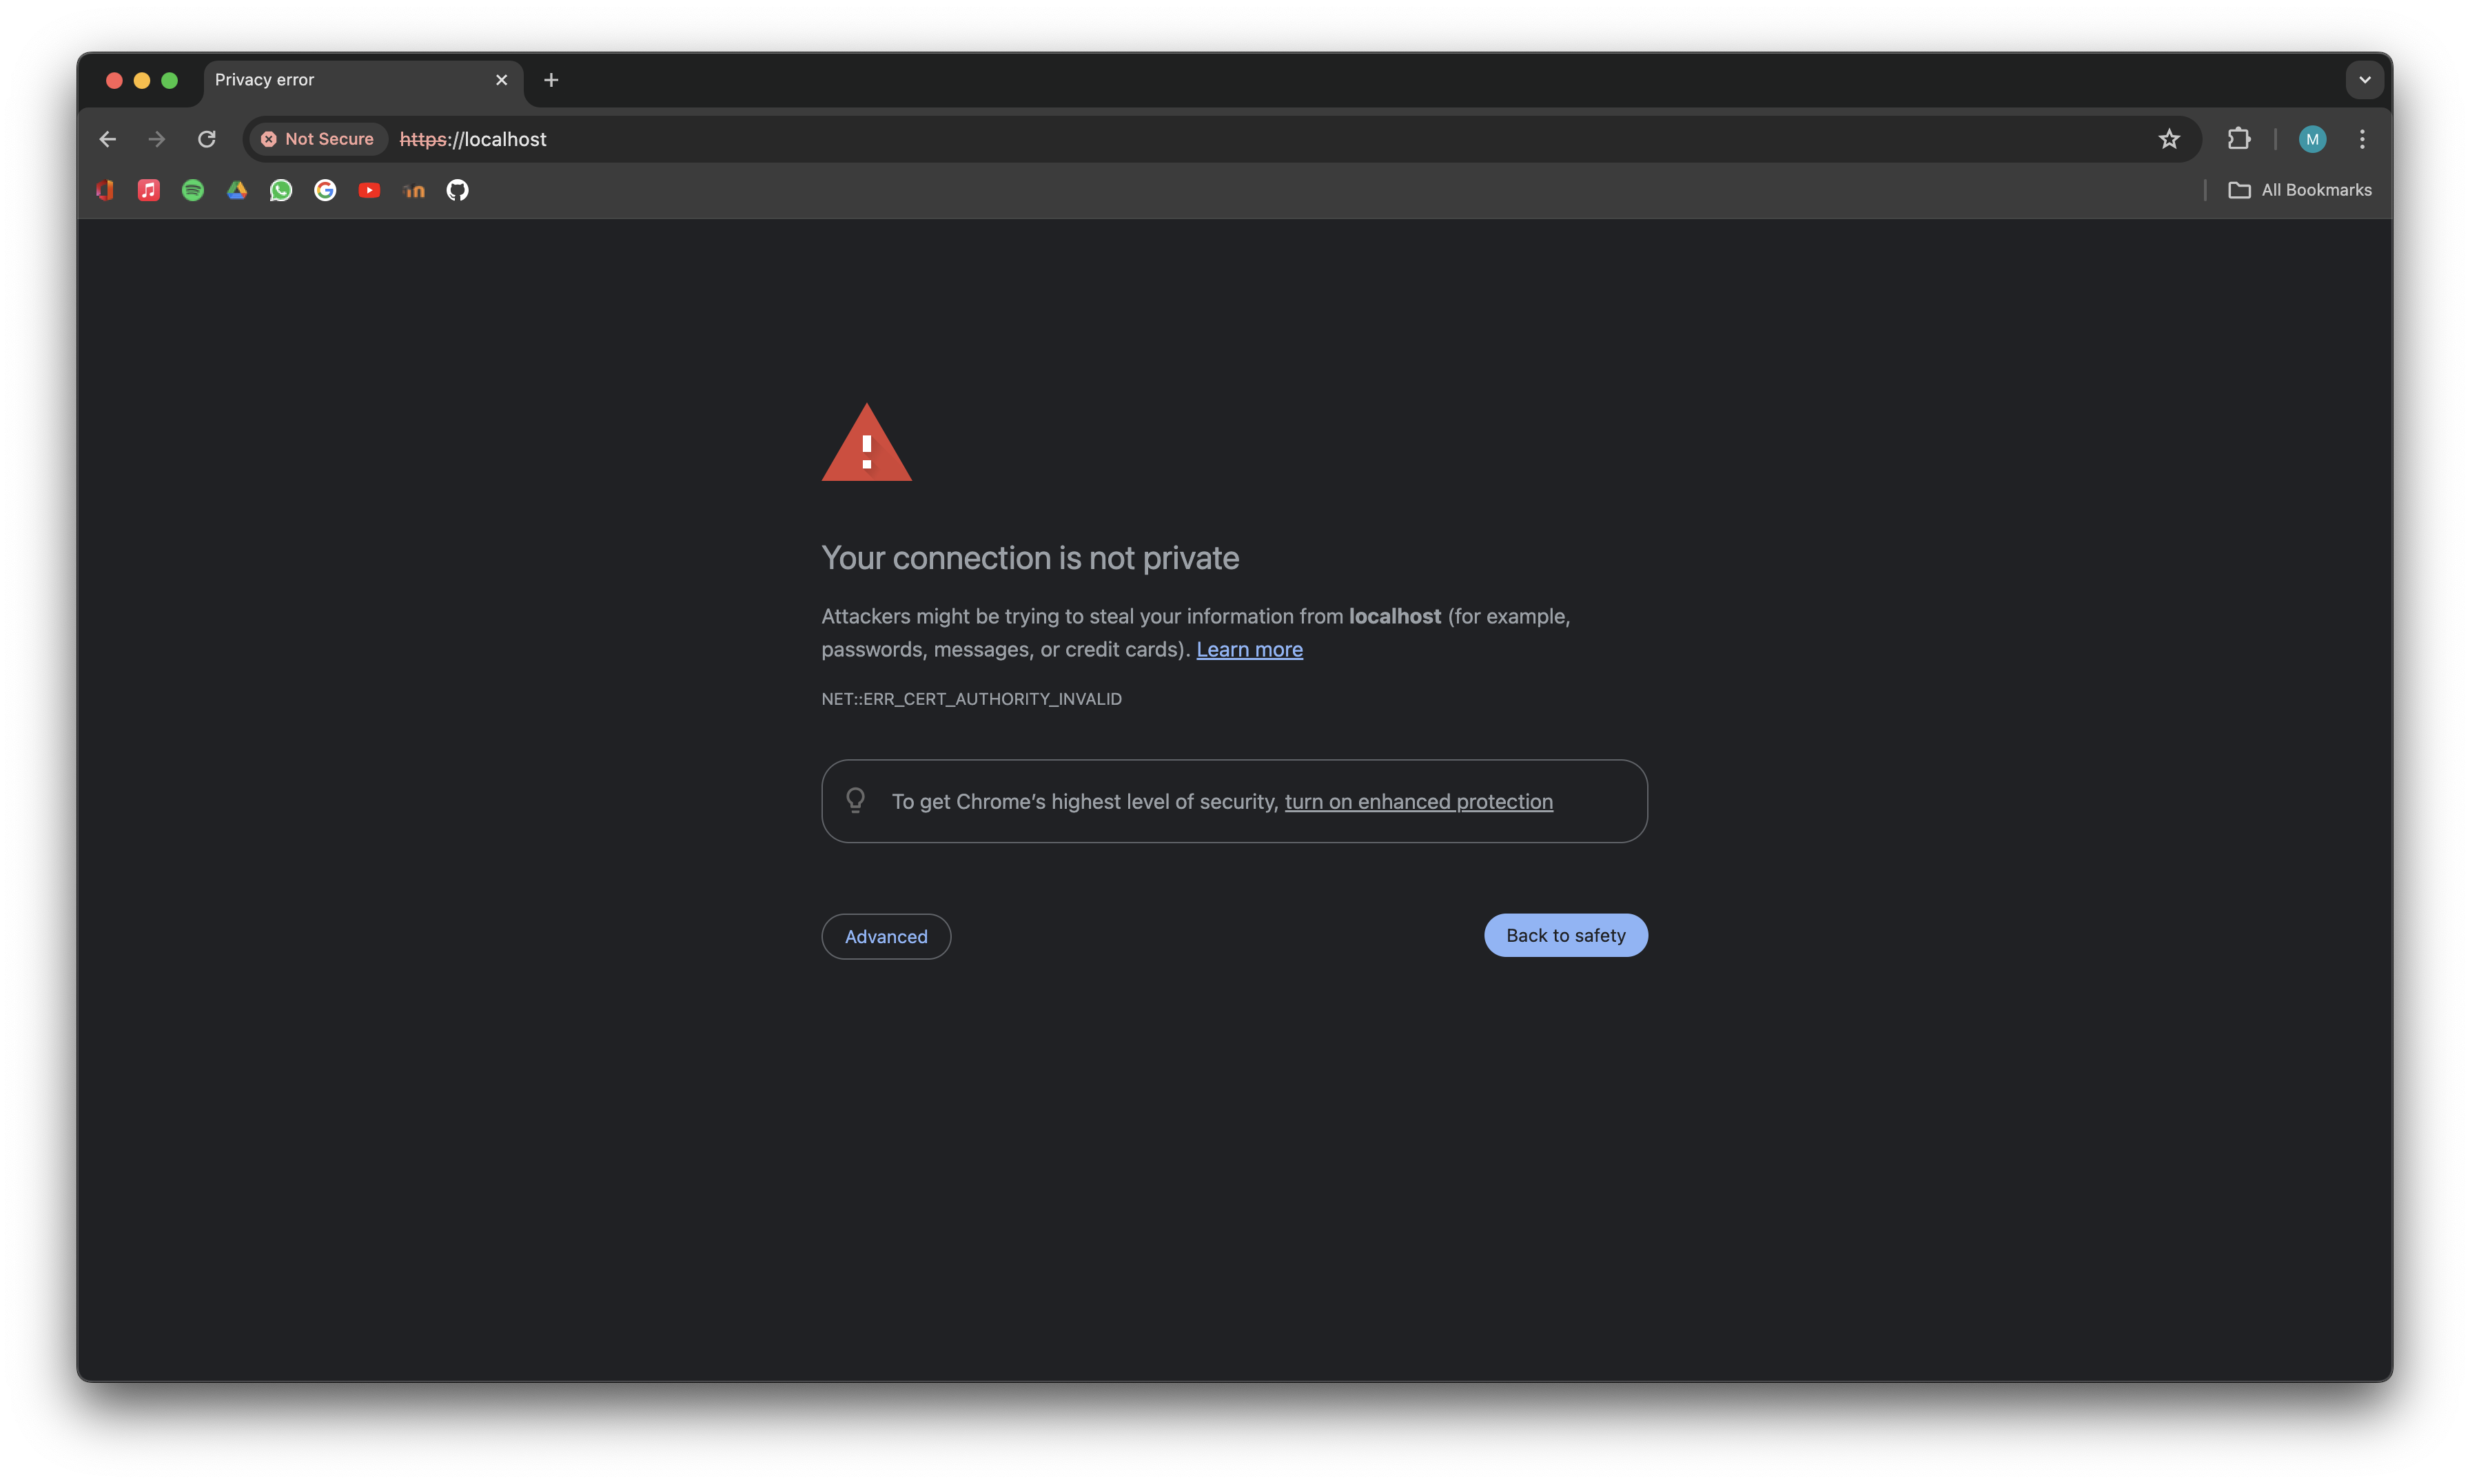
\includegraphics[width=1\linewidth]{conNotPrivate.png}
    \caption{Mensaje de conexión privada}
\end{figure}
\paragraph{}
Este mensaje es normal que nos aparezca ya que nuestro certificado no es validado por una entidad externa, ya que nosotros hemos generado un certificado auto firmado el cual simula una conexión segura HTTPS sin ningún coste adicional. Por lo tanto si pulsamos en \textit{Advanced} y luego en ir a la página se nos abrirá nuestra web con el certificado SSL.

\subsection{Resultados y análisis}
En primer lugar, se ha configurado la página web para que se pueda mostrar en 3 idiomas: Español, Inglés(UK) e Inglés(US), ya que son los 3 idiomas que se hablan donde se ubican las compañías. 
\newpage
\begin{figure}[h]
    \centering
    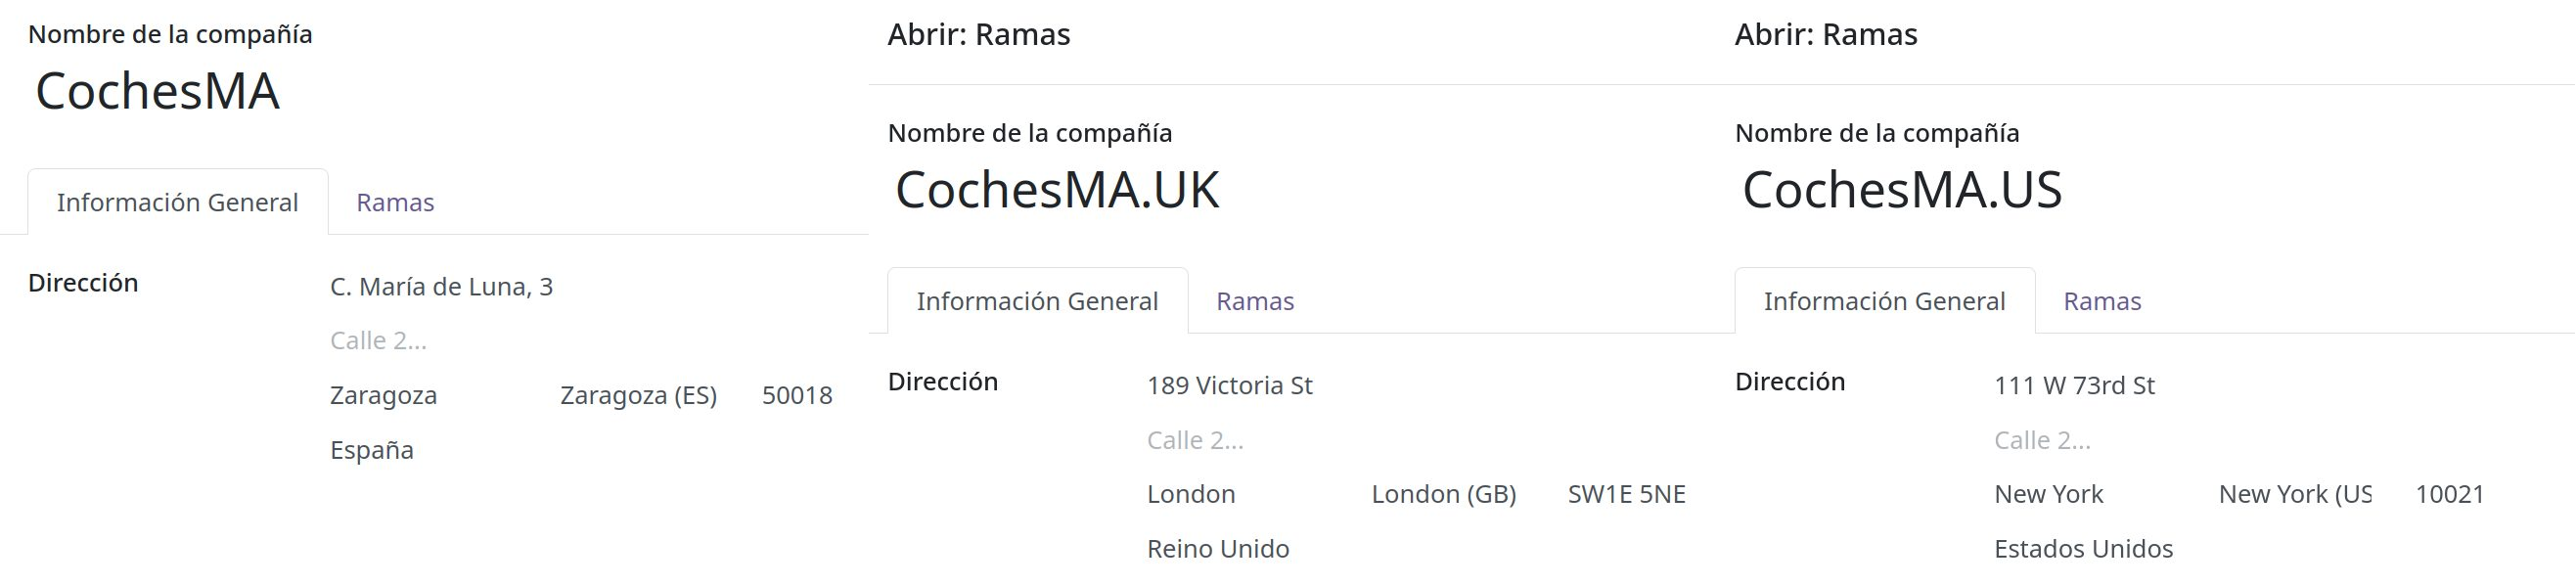
\includegraphics[width=1\linewidth]{fotosConfiguración/ubicaciones.jpg}
    \caption{Ubicación de las empresas}
    \label{fig:enter-label}
\end{figure}
Se ha personalizado la web para que contenga el logo, el nombre, la misión, el correo electrónico, la localización y el número de teléfono y se ha cambiado los colores a blanco y a azul.
\begin{figure}[h]
    \centering
    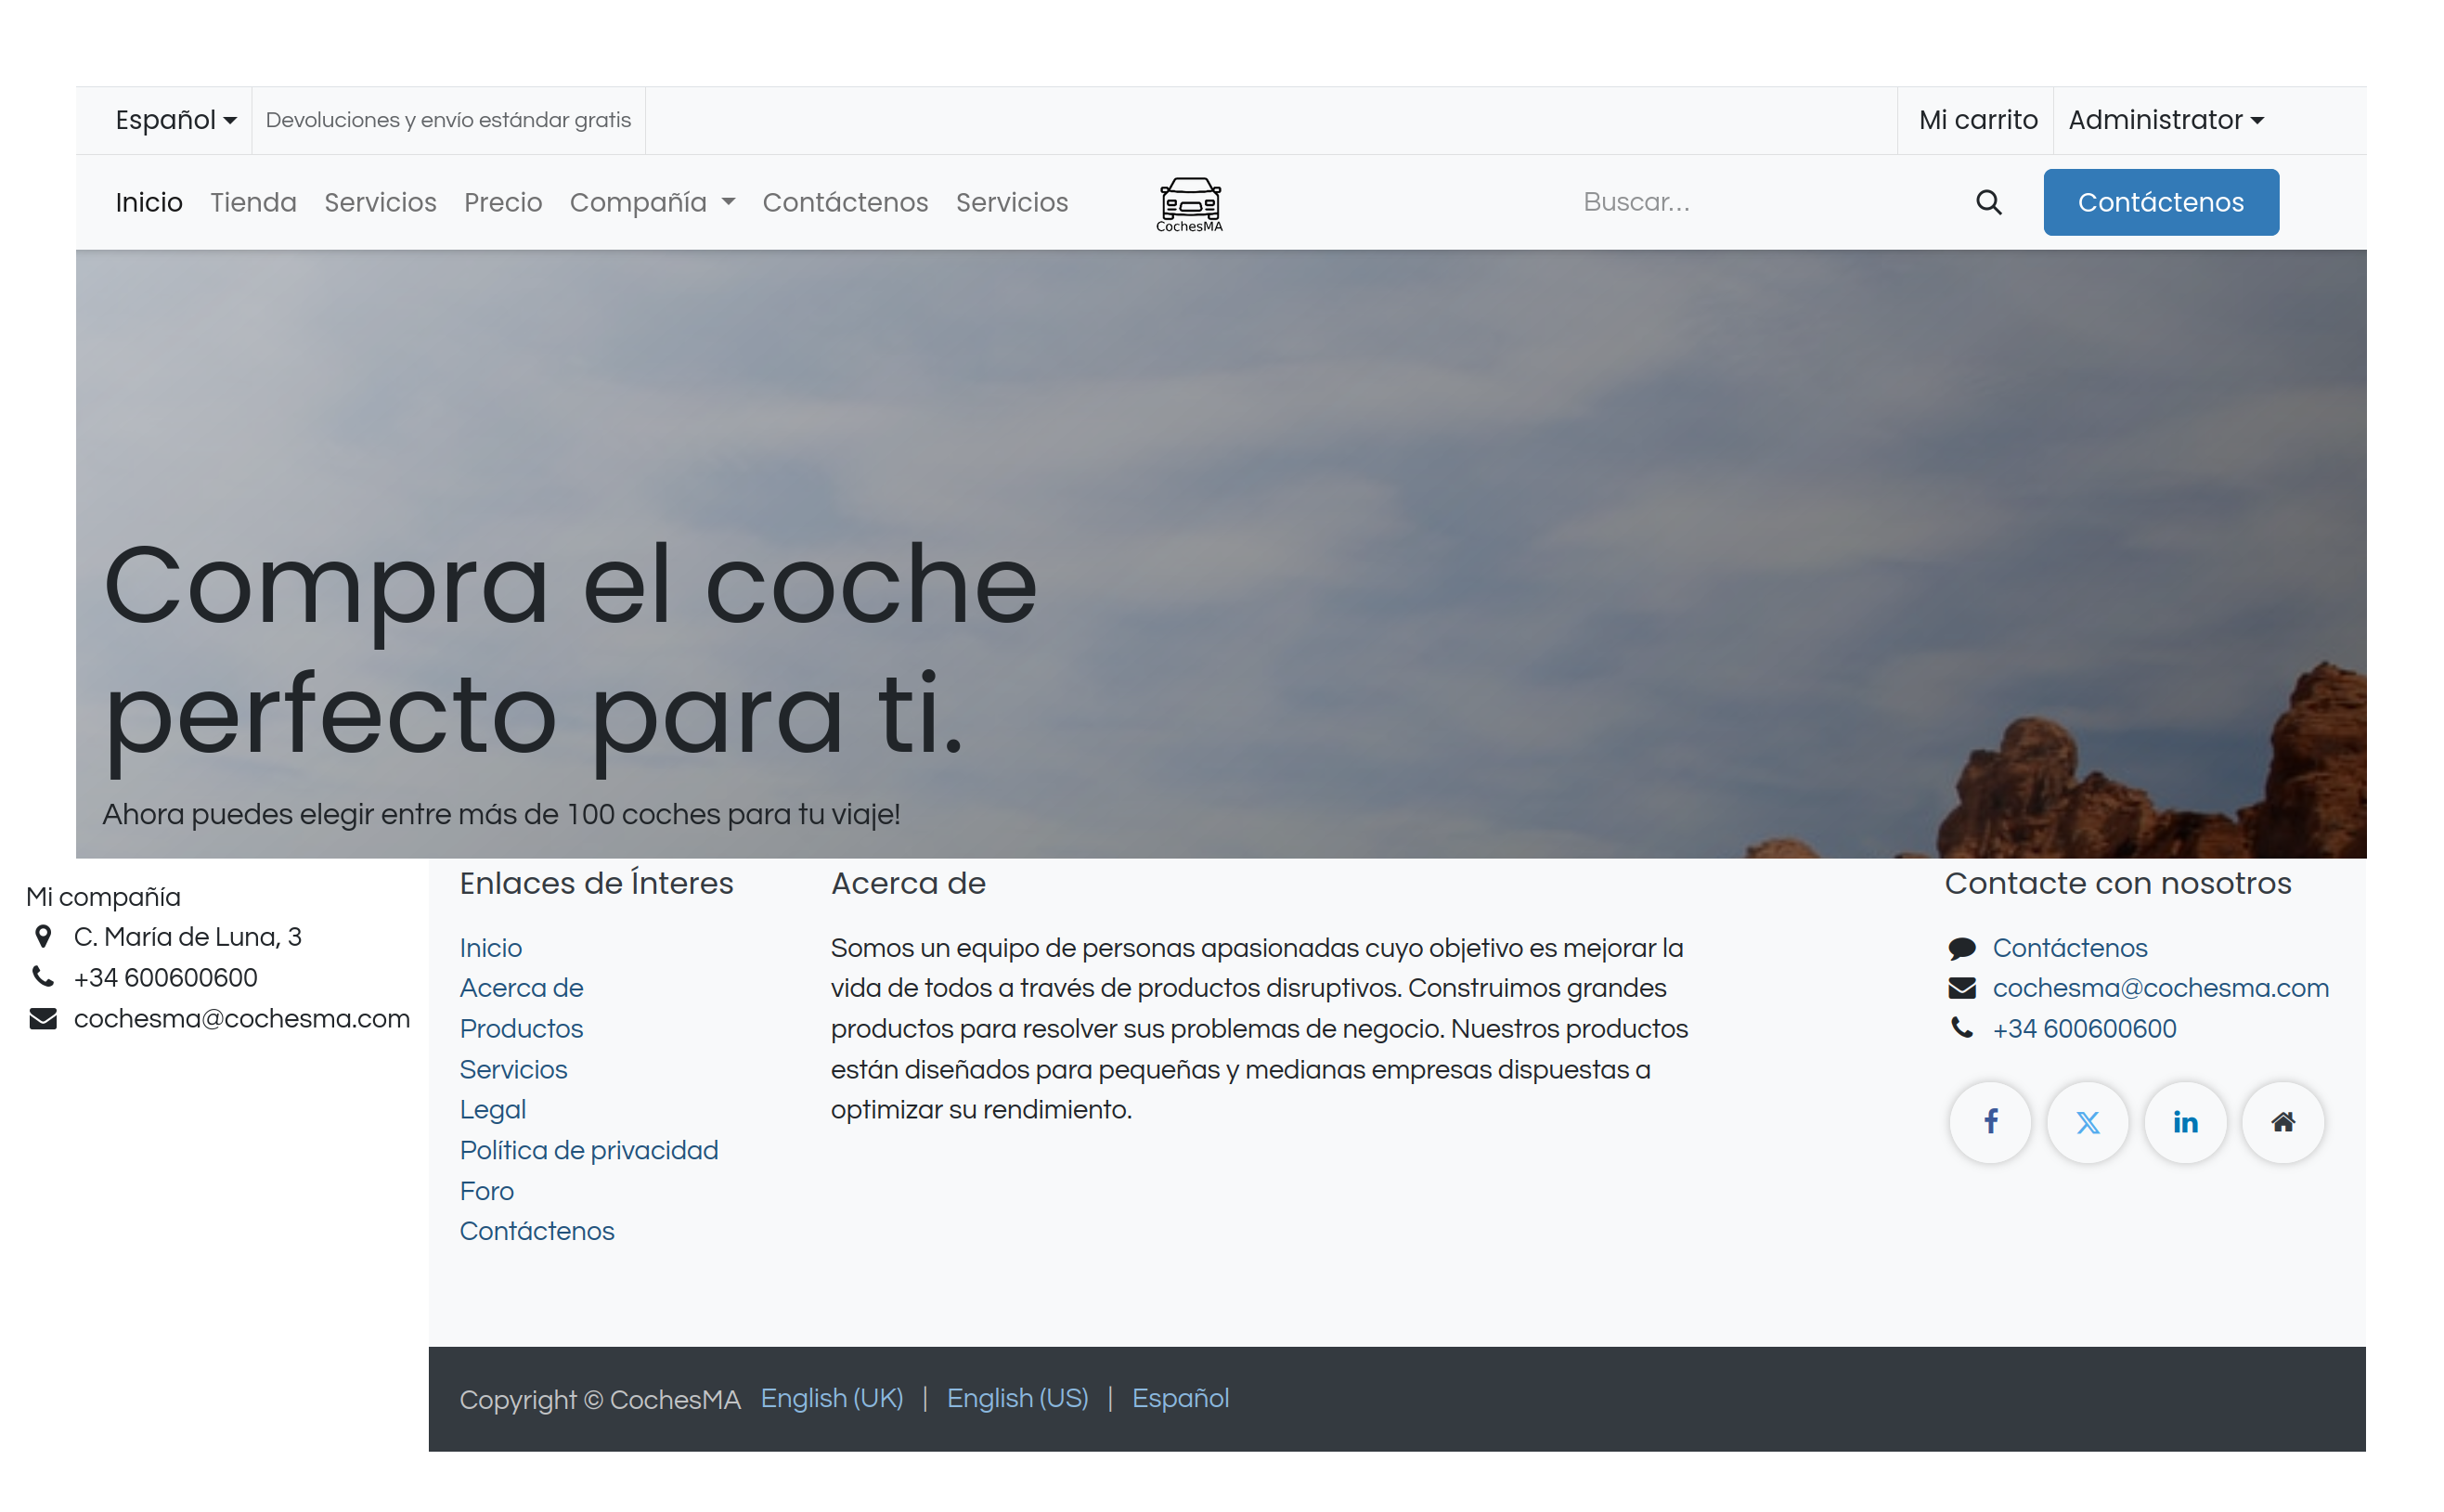
\includegraphics[width=1\linewidth]{fotosConfiguración/personalización.png}
    \caption{Personalizaciones de la web}
    \label{fig:enter-label}
\end{figure}

Además, se han realizado optimizaciones de SEO, para mejorar el ranking de la web en Google, para ello se ha añadido el logo, un título y una descripción adecuada y se han añadido palabras clave como alquiler, coche, viaje y en inglés, rent, car.
\newpage
\begin{figure}[h]
    \centering
    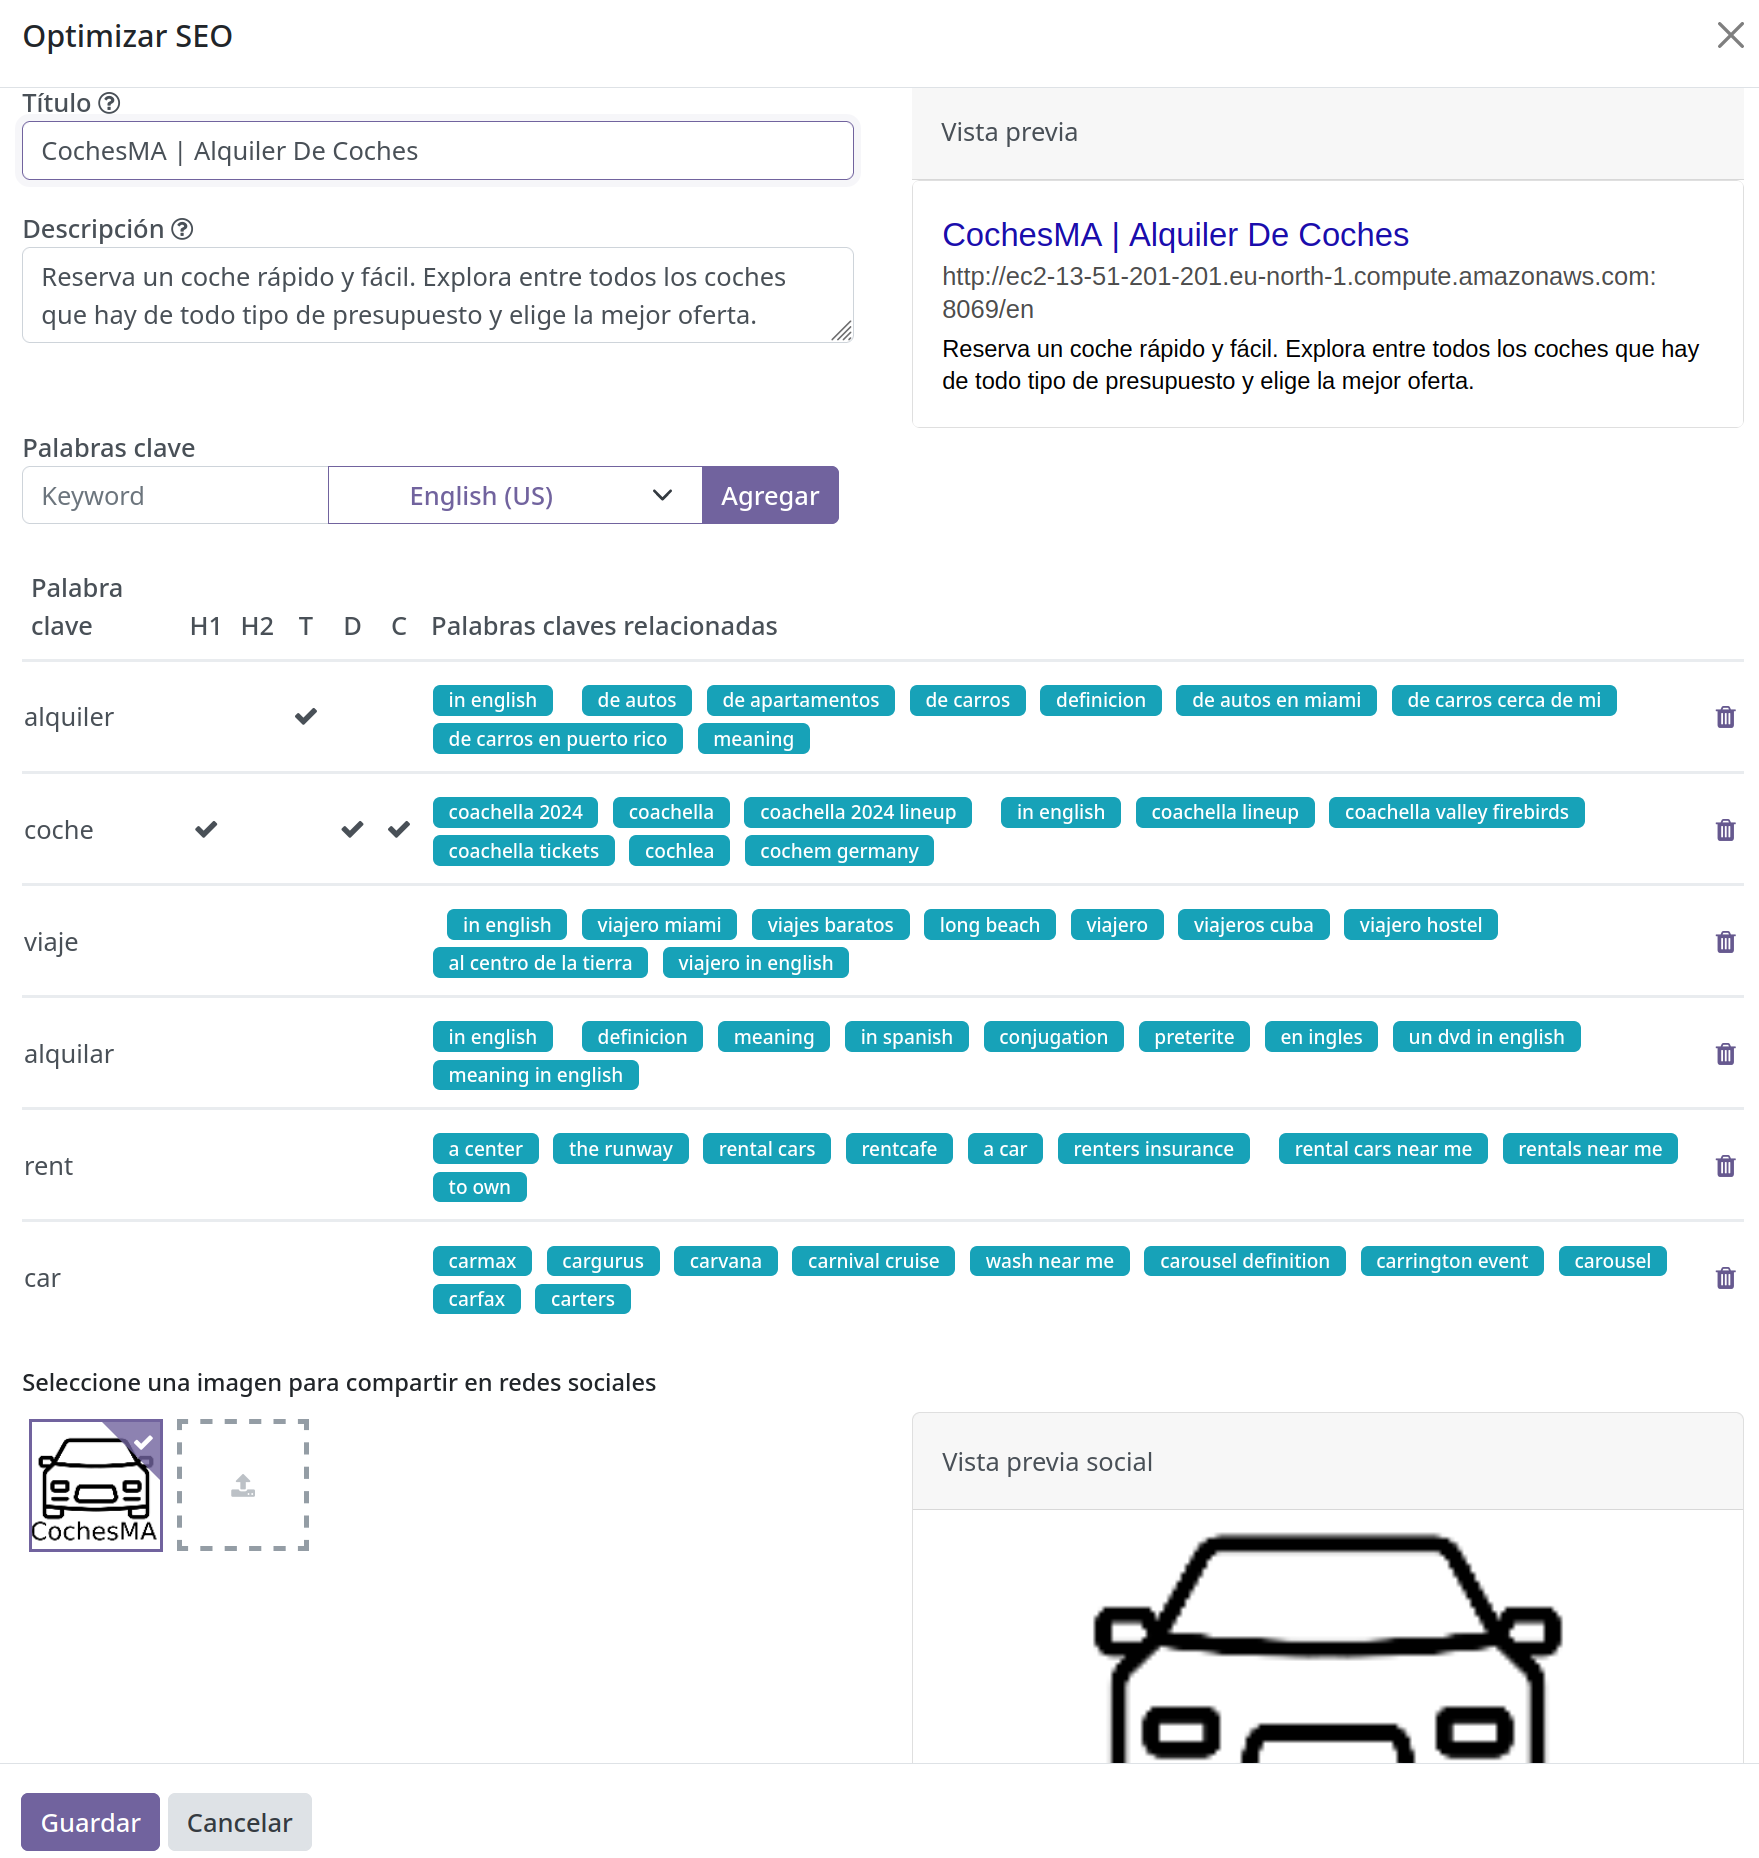
\includegraphics[width=1\linewidth]{fotosConfiguración/seo.png}
    \caption{Configuración del SEO}
    \label{fig:enter-label}
\end{figure}

\paragraph{}
Por último, hemos logrado implementar un servidor SSL localmente que nos permite acceder a nuestra web desde un dominio propio con conexión segura utilizando un servidor Nginx. 
\begin{figure}[h]
    \centering
    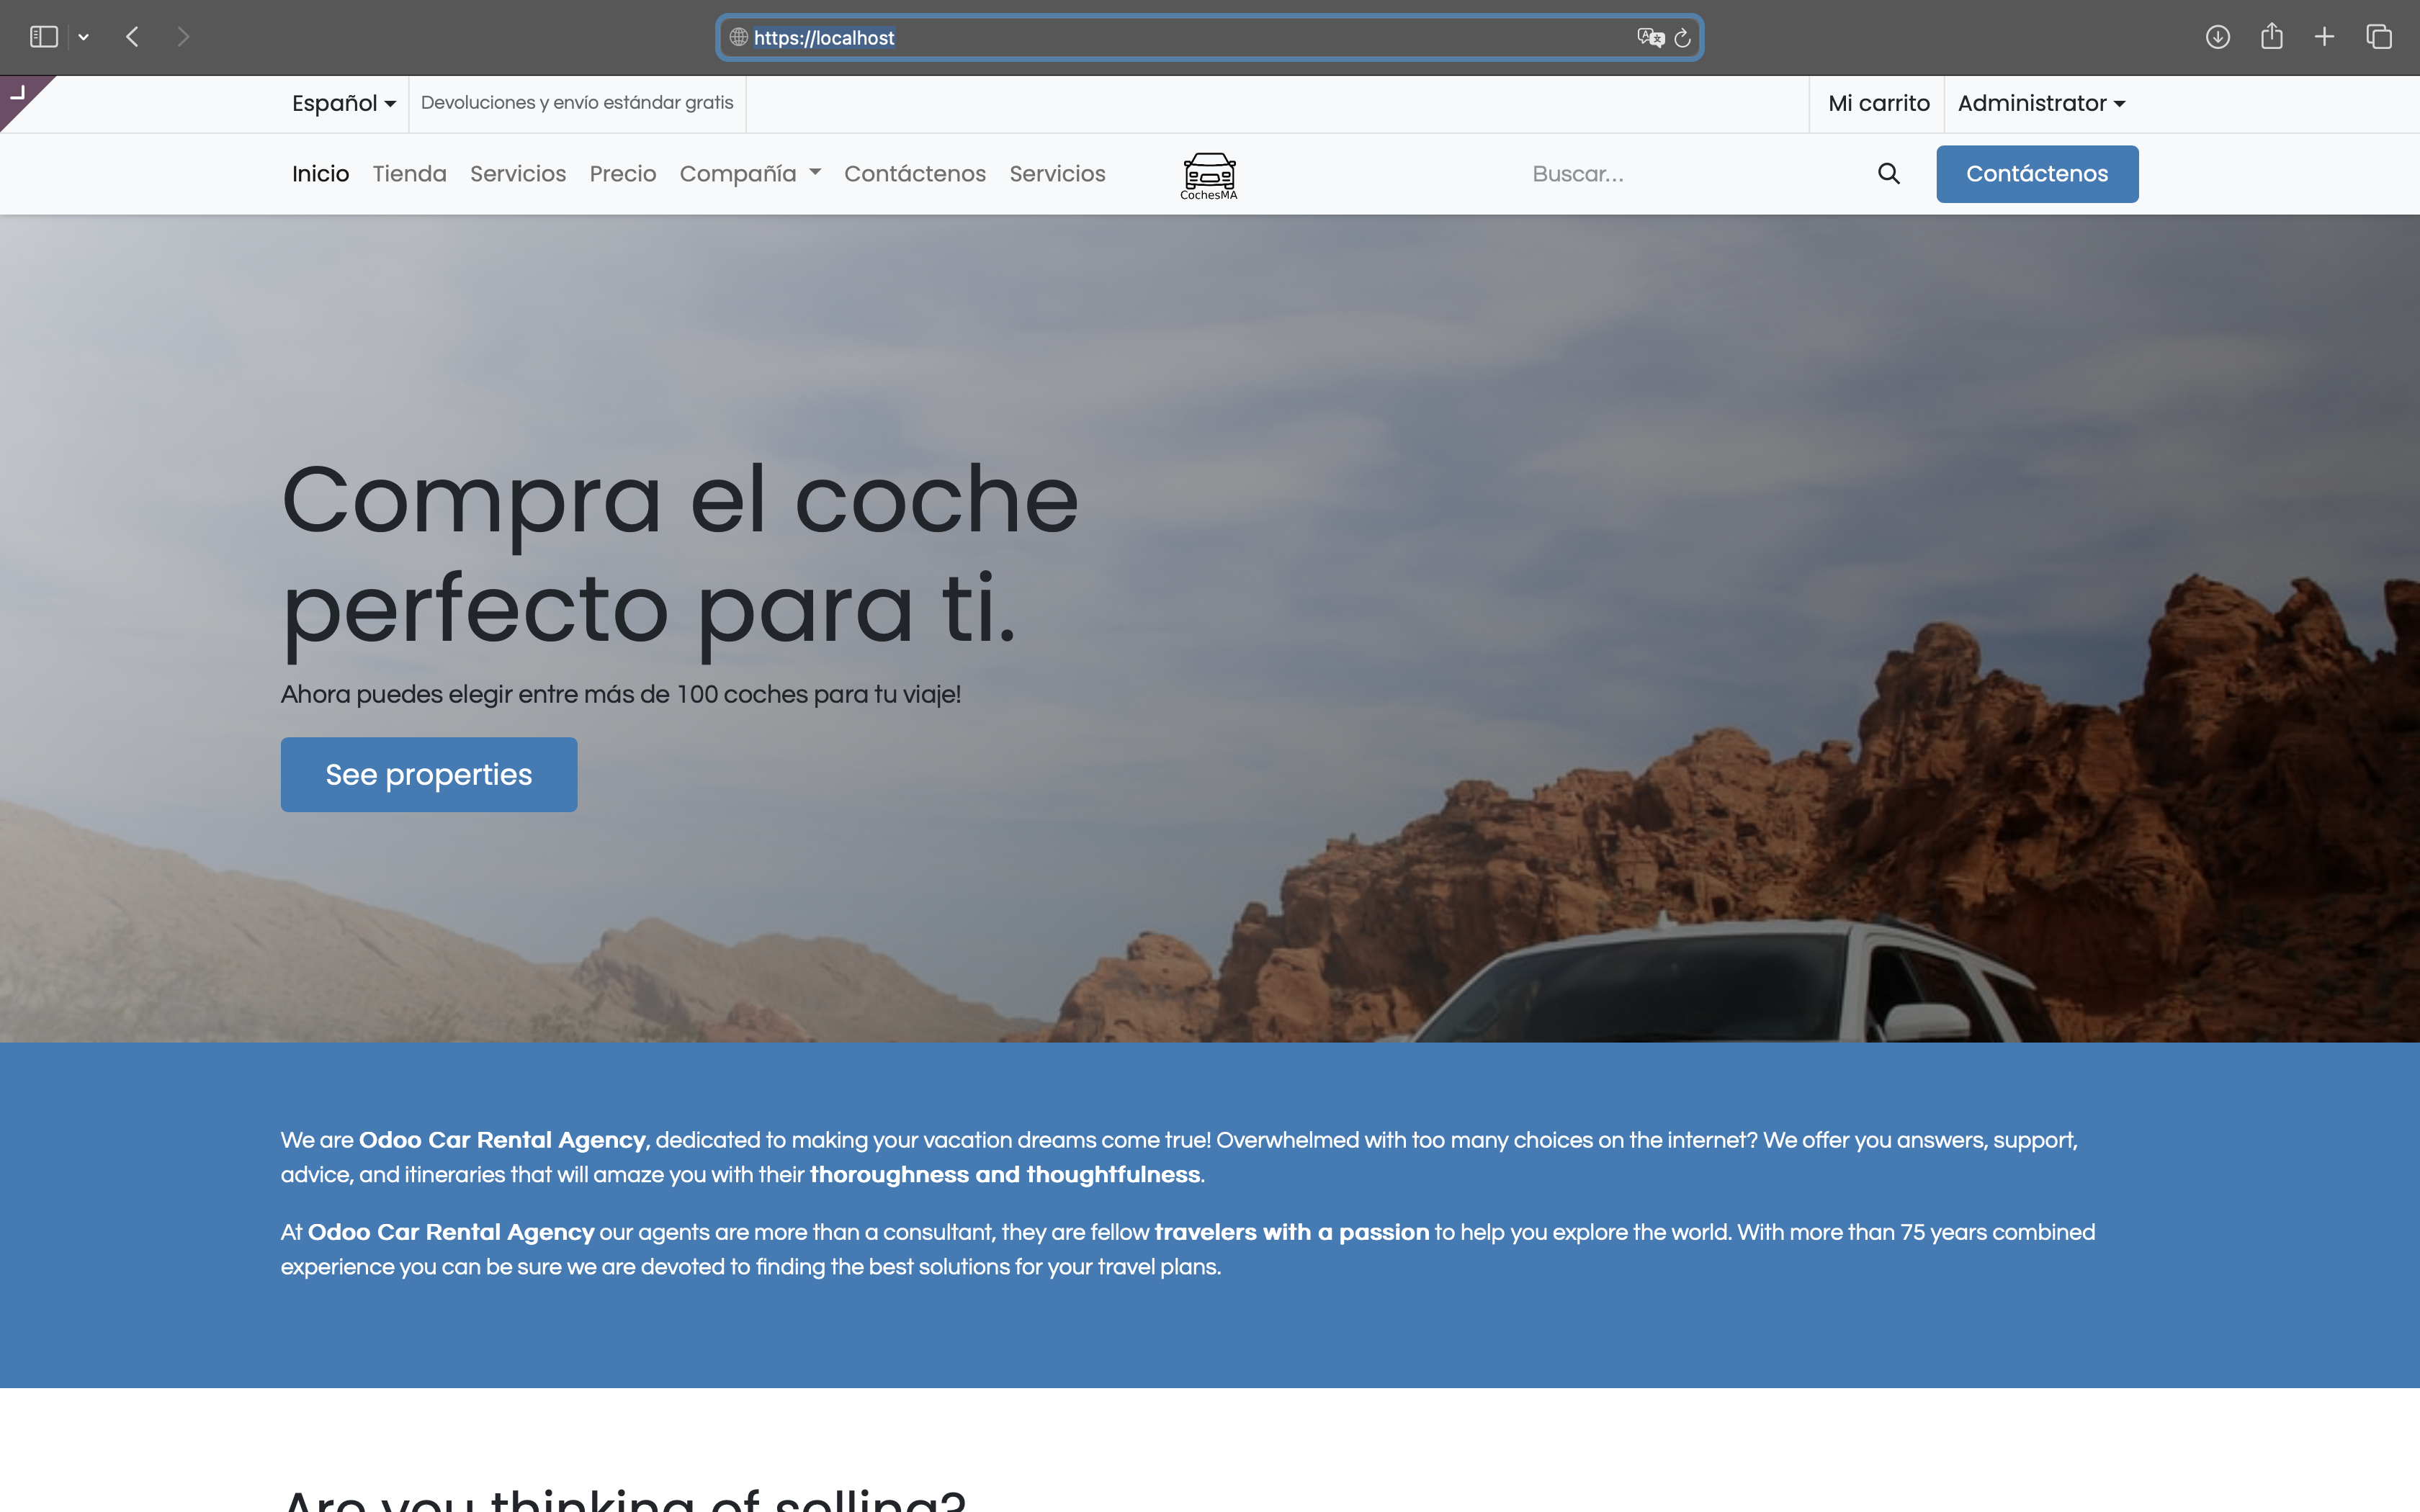
\includegraphics[width=1\linewidth]{SSL.png}
    \caption{Captura de pantalla del navegador con nuestra web en un dominio propio}
\end{figure}
\subsection{Conclusiones}
\paragraph{}
En cuanto al sistema multilingüe es sencillo la configuración pero tiene ciertas limitaciones, por ejemplo, no se ha conseguido que se traduzca todo el contenido de la página web como aquella información añadida manualmente. Aunque, permite traducir la mayoría de la pagina web lo suficiente para que se pueda navegar y realizar el servicio deseado. 
\paragraph{}
El proceso de personalización de la web es sencillo, intituitivo y ofrece una gran libertad posibilitando editar la página web y adecuarla a las necesidades de la compañía. En cuanto a la optimización del SEO es correcta permitiendo escalar la promoción de la web en el ranking del buscador. 
\paragraph{}
En referencia a la implementación de un servidor SSL para acceder desde un dominio propio con conexión HTTPS es muy sencillo y rápido. Únicamente se ha tenido que generar las claves, modificar el fichero utilizado para su configuración y añadir un segundo fichero. Este proceso sería similar para hacer en el entorno de despliegue. La gran diferencia es que el certificado utilizado no se puede auto firmar y se debe comprar para que sea validado por una entidad externa y los navegadores confíen en él.



%\section{Configuración técnica}
%\subsection{Copia de seguridad}
%\subsubsection{Autoevaluación}

%\subsubsection{Introducción}
%Este apartado aborda la gestión de las copias de seguridad en Odoo. Se va a hacer una evaluación de la configuración que ofrece para gestionar las bases de datos, la posibilidad de transferir los datos de Odoo de una instancia a otra y la capacidad de crear scripts para automatizar las copias de seguridad, las cuáles van a ser almacenadas en la nube.
%\subsubsection{Metodología}
%El primer paso que se ha realizado ha sido dirigirnos a la siguiente dirección en el navegador \textit{http://ec2-13-51-201-201.eu-north-1.compute.amazonaws.com:8069/web/database/manager}. Se ha hecho click en \textit{Set Master Password} y se ha introducido una contraseña que será necesaria en las operaciones que se van a realizar en este módulo. A continuación, Odoo ofrece una opción para crear una nueva base de datos, para ello se ha hecho click en \textit{Create Database} y se ha rellenado el formulario. Tras pulsar el botón de crear hay que esperar hasta que nos ha redirigido al inicio de sesión, una vez iniciado sesión con la información introducida anteriormente, ya puedes acceder a Odoo. También, ofrece una opción para duplicar una base de datos, para ello se ha pulsado en \textit{Duplicate} en la base de datos que se quiere duplicar y se ha introducido el nuevo nombre y la contraseña maestra, tras unos segundos se ha comprobado que se ha mostrado una nueva entrada en la lista de bases de datos, la cual tendrá la misma información que la original. Odoo nos da la posibilidad de eliminar bases de datos. En la lista se ha pulsado el botón \textit{Delete} del elemento que se quiere borrar y tras introducir la contraseña maestra se ha eliminado la base de datos. Por último, Odoo ofrece la posibilidad de realizar una copia de seguridad de las bases de datos. Para probar esta funcionalidad se ha hecho click en \textit{Backup} en la base de datos que se quiere realizar y se ha seleccionado el formato zip. Cómo resultado se descarga en la máquina un zip con la información de la base de datos. La capacidad de exportar la información junto con la posibilidad que ofrece Odoo de restaurar una base de datos, nos permite realizar transferencias de las bases de datos. Para comprobarlo se ha hecho una copia de seguridad de una de ellas como se ha explicado anteriormente y se ha enviado por WhatsApp. En otra máquina donde se tiene instalado Odoo, se ha accedido a WhatsApp y se ha descargado el zip. A continuación, nos hemos dirigido a \textit{http://localhost:8069/web/database/manager} y se ha hecho click en \textit{Restore Database}, se ha introducido la contraseña maestra y el nombre, se ha activado la opción de que la base de datos es una copia y se ha seleccionado el zip que contiene la información. Como resultado se ha creado una nueva entrada en la lista de bases de datos la cual contiene la información que se tenía en la otra máquina.
%\subsubsection{Resultados y análisis}
%Se ha conseguido realizar en Odoo la creación, eliminación, duplicación y copia de seguridad de una base de datos. Además, se ha conseguido transferir una base de datos de una instancia de Odoo a otra, mediante realización de una copia de seguridad de una base de datos y la restauración de la misma. 
%\subsubsection{Conclusiones}

%\newpage
%\subsection{Correo electrónico}
%\subsubsection{Autoevaluación}
%8
%\subsubsection{Introducción}
%Con el objetivo de permitir la comunicación de la empresa mediante Odoo se ha configurado un servidor de correo electrónico tanto saliente para poder enviar correos como entrante para poder recibirlos.
%\subsubsection{Metodología}
%Para crear un servidor SMTP y poder enviar correos a través de él, hay que ir a los ajustes de opciones generales, entrar en el menú de Servidores de correo saliente y crear un nuevo servidor. En este caso, se ha utilizado autentificación OAuth de Gmail, hay que asegurarse que se ha introducido \textit{odoo.com} en el campo Filtro DESDE, TLS como encriptación, \textit{smtp.gmail.com} como servidor SMTP y puerto 587. Se ha decidido utilizar un correo de UNIZAR para llevar a cabo la conexión con Gmail por lo que se ha puesto ese correo en el campo de nombre de usuario. A continuación, hay que insertar el ID y el Numero secreto en \textit{Usar un servidor de Gmail} en las opciones generales de los ajustes. Para ello, se ha ido a la siguiente web \textit{https://console.cloud.google.com/apis/} se ha iniciado sesión en gmail y se ha creado un nuevo proyecto llamado Odoo. Primero, en pantalla de consentimiento de OAuth se ha elegido el tipo de usuario externo, se han rellenao los formularios necesarios, cabe destacar que hay que añadir como dominio autorizado \textit{odoo.com}. A continuación, se ha ido al menú \textit{Crear credenciales} y se ha seleccionado la opción OAuth client ID. En este menú se ha elegido la opción \textit{Aplicación web} y se ha añadido como URIS de redirección autorizadas \textit{http://ec2-13-51-201-201.eu-north-1.compute.amazonaws.com:8069/google\_gmail/confirm} . En la misma pantalla se mostrará el \textit{ID} y \textit{Secreto} con los que hay que rellenar los campos en Odoo. En la pantalla del servidor de correo que se estaba creando la prueba de conexión será exitosa. Por otro lado, el proceso de añadir un servidor de correo entrante es similar. Cabe destacar que en el campo de nombre del servidor se ha introducido \textit{imap.gmail.com} y se ha activado la opción SSL/TLS. Para llevar a cabo el proceso de envío de un correo electrónico desde Odoo y probar el servidor de salida se ha instalado el módulo Contactos. En este módulo se muestra todos los contactos de empleados, empresas, individuos que se ha tenido. Si se hace click en un contacto, se podrá ver a la derecha un chat en el que se ha escrito un correo y se ha enviado.
%\subsubsection{Resultados y análisis}
%\subsubsection{Conclusiones}
